% Arjun as a Boolean-Function Synthesis Engine -- 15 minute talk
% Compile with:  pdflatex arjun_synth.tex   (run twice for the ToC/refs)
\documentclass[aspectratio=169]{beamer}

\usetheme{Boadilla}
\usecolortheme{whale}
\setbeamertemplate{navigation symbols}{}
\setbeamertemplate{caption}{\insertcaption}
\setbeamertemplate{bibliography item}{}

\usepackage{booktabs}
\usepackage{tikz}
\usetikzlibrary{arrows.meta,positioning,shapes.geometric,fit,backgrounds}
\usepackage{graphicx}

% ---- colours -------------------------------------------------------------
\definecolor{stageA}{RGB}{ 70,115,170}   % cheap defs (autarky, extend)
\definecolor{stageB}{RGB}{ 89,161, 79}   % SAT-per-var defs (backward, unate)
\definecolor{stageC}{RGB}{225,140, 43}   % Manthan
\definecolor{ioBox}{RGB}{ 90, 90, 90}
\definecolor{hl}{RGB}{200, 60, 60}

% ---- flow-chart node styles ---------------------------------------------
\tikzset{
  io/.style   ={rectangle, rounded corners=1pt, draw=ioBox, fill=ioBox!12,
                 text width=88mm, align=center, font=\scriptsize, inner sep=2.6pt},
  sA/.style   ={rectangle, rounded corners=3pt, draw=stageA, fill=stageA!15,
                 text width=88mm, align=left, font=\scriptsize, inner sep=3pt},
  sB/.style   ={rectangle, rounded corners=3pt, draw=stageB, fill=stageB!15,
                 text width=88mm, align=left, font=\scriptsize, inner sep=3pt},
  sC/.style   ={rectangle, rounded corners=3pt, draw=stageC, fill=stageC!18,
                 text width=88mm, align=left, font=\scriptsize, inner sep=3pt},
  fl/.style   ={-{Stealth[length=1.8mm]}, semithick, draw=ioBox},
  note/.style ={font=\tiny\itshape, align=left, text width=30mm},
}

\title[Arjun as a Synthesis Engine]{Arjun as a Boolean-Function Synthesis Engine}
\subtitle{From Puura-simplified CNF to an AIG that defines every output}
\author{Mate Soos}
\date{\today}

\begin{document}

% =========================================================================
\begin{frame}[plain]
  \titlepage
  \begin{center}\scriptsize
  Synthesising Boolean functions $Y = f(X)$ from a relation
  $\exists Y.\, F(X,Y)$ \\
  --- a counterexample-guided pipeline built on CryptoMiniSat \& CaDiCaL.
  \end{center}
\end{frame}

% =========================================================================
\begin{frame}{The synthesis problem}
  \textbf{Input:} a CNF $F(X, Y)$ together with a partition of the
  variables --- the user marks which are \emph{inputs} $X$ and which are
  \emph{outputs} (to-define) $Y$.
  \medskip

  \textbf{Output:} an \alert{AIG} (And--Inverter Graph) that gives every
  $y_i \in Y$ as a Boolean function $y_i = f_i(X, y_{<i})$ such that
  $F(X, f(X))$ holds whenever $\exists Y.\, F(X,Y)$ does.
  \medskip

  \begin{block}{Where the formula comes from}
  Typical sources are \textbf{QBF} (the $\forall X \exists Y.\, F$ fragment used
  in Skolem-function synthesis~\cite{niemetz2012b}), \textbf{reactive
  synthesis} from temporal specs, and \textbf{circuit repair / don't-care
  optimisation}~\cite{john2015efficient}.
  \end{block}
  \medskip

  Arjun runs as a tool: \texttt{./arjun --synth input.cnf}. It first
  invokes \textbf{Puura}~\cite{korhonen2021integrating, soos2019bird}
  (CNF simplification --- \emph{not} covered today) and then attacks the
  \emph{synthesis} problem on the simplified formula.
\end{frame}

% =========================================================================
\begin{frame}{Three kinds of variables --- the only abstraction you need}
  Throughout the run Arjun classifies every CNF variable into one of three
  buckets, recorded on the \texttt{SimplifiedCNF} container
  (\texttt{src/arjun.cpp}):
  \medskip

  \begin{description}\setlength{\itemsep}{4pt}
    \item[\textcolor{stageA}{\textbf{input}}] vars in $X$ --- the
      free inputs. Their value is whatever the user / environment hands
      us; we never define them.
    \item[\textcolor{stageB}{\textbf{to-define}}] vars in $Y$ for which we
      still need to produce an AIG $f_i$. The set shrinks monotonically as
      the pipeline progresses.
    \item[\textcolor{stageC}{\textbf{backward-defined}}] vars
      $y_i \in Y$ that already have an AIG --- ``backward'' in the sense
      that we proved $y_i$ is determined by inputs and earlier outputs.
  \end{description}
  \medskip

  \textbf{Invariant:} every stage's job is to move variables out of
  \emph{to-define} and into \emph{backward-defined}, with a verified AIG
  attached. When \texttt{to\_define} is empty we are done
  (\texttt{cnf.synth\_done()}).
  \medskip

  \begin{exampleblock}{\small Log header (bobtuint07neg)}
  \scriptsize
  \texttt{Num input vars: 432 \; Num to-define vars: 1204 \;
  Num backward-synth-defined vars: 0}
  \end{exampleblock}
\end{frame}

% =========================================================================
\begin{frame}{The synthesis pipeline}
\vspace{-2mm}
\begin{center}
\begin{tikzpicture}[node distance=1.7mm]

\node[io] (in) {\texttt{Puura-simplified CNF} \;+\; \texttt{c p show} (= inputs)};

\node[sA, below=of in] (s1)
 {\textbf{1. Autarky} {\tiny (\texttt{--autarky}, on by default; \texttt{autarky.cpp})}\\
  {\tiny find a partial assignment that satisfies every clause it touches \cite{liffiton2008}}};

\node[sB, below=of s1] (s2)
 {\textbf{2. Extend (UNSAT-define)} {\tiny (\texttt{--extend}, on by default; \texttt{extend.cpp})}\\
  {\tiny per-var SAT call on a doubled CNF; UNSAT $\Rightarrow$ var is determined by inputs alone}};

\node[sB, below=of s2] (s3)
 {\textbf{3. Backward-round-synth} {\tiny (\texttt{--minimize}, on by default; \texttt{backward.cpp})}\\
  {\tiny same trick, but lets the var depend on \emph{any} earlier var --- not just inputs}};

\node[sB, below=of s3] (s4)
 {\textbf{4. Unate / definition probe} {\tiny (\texttt{--unatedef}, on by default; \texttt{unate\_def.cpp})}\\
  {\tiny ``def'' part: $y_i$ forced to a constant. \;
   ``conditional'' part: $y_i = \pm L$ for some literal $L$}};

\node[sC, below=of s4] (s5)
 {\textbf{5. Manthan} {\tiny (always runs last; \texttt{manthan.cpp, synth.cpp})}\\
  {\tiny BVE-based initial guess $\rightarrow$ counterexample-guided repair (CEGAR) \cite{golia2020manthan, golia2021engineering}}};

\node[io, below=of s5] (out)
 {AIG that defines every to-define variable \;($-$final.aig)};

\foreach \a/\b in {in/s0, s0/s1, s1/s2, s2/s3, s3/s4, s4/s5, s5/out}
  \draw[fl] (\a) -- (\b);

\node[note, right=2mm of s1.east, text=stageA] {cheap,\\global};
\node[note, right=2mm of s3.east, text=stageB] {one SAT call\\per variable};
\node[note, right=2mm of s5.east, text=stageC] {CEGAR loop\\the hard cases};

\end{tikzpicture}
\end{center}
\vspace{-1mm}
\scriptsize Stage ordering and \texttt{check\_stage} debug hooks live in
\texttt{src/main.cpp}; each stage writes a \texttt{-STAGE.aig} dump under \texttt{--debugsynth}.
\end{frame}

% =========================================================================
\begin{frame}{Stage 1 --- Autarky}
  \textbf{Autarky}~\cite{liffiton2008}. An \emph{autarky} is a partial
  assignment that satisfies every clause it \emph{touches}. Those clauses
  and the variables in them can be deleted without changing $\exists Y.\, F$,
  because we can always extend any partial model with the autarky.
  \medskip

  \begin{exampleblock}{\small Log: autarky on bobtuint07neg}
  \scriptsize
  \texttt{[autarky] Done. do\_autarky found autarkies: 0 defined: 0 \\
   still to-define: 353}
  \end{exampleblock}
  \medskip
  Autarky often finds nothing on QBF benchmarks but is essentially free, so
  it stays on by default.
\end{frame}

% =========================================================================
\begin{frame}{Stage 2 --- Extend (UNSAT-define): the duplication trick}
  \textbf{Goal:} prove that a single output $y$ is fully determined by the
  \emph{inputs alone} --- and, if it is, extract the AIG defining it.
  \medskip

  \textbf{The construction} (\texttt{extend.cpp}, also used by
  \cite{soos2020bird}, \cite{durand2025fbcounting}):
  \begin{enumerate}\setlength{\itemsep}{1pt}
    \item Build the \alert{doubled CNF} $F(X, Y_1) \wedge F(X, Y_2)$ ---
          inputs $X$ are shared, every non-input has two copies.
    \item For each candidate $y$, ask the SAT solver:
          \emph{can $y_1 \neq y_2$ while all inputs agree?}
          If \textbf{UNSAT}: $y$ is a function of $X$.
  \end{enumerate}
  \medskip

  \textbf{From UNSAT to AIG.} A CaDiCaL proof tracer reconstructs a
  \alert{McMillan interpolant} over the input vars from the refutation
  proof. The interpolant \emph{is} the AIG definition of $y$
  (\texttt{interpolant.cpp}; idea: \cite{mcmillan2003interpolation},
  \cite{jiang2009interpolating}).
  \medskip

  \begin{exampleblock}{\small Log: extend on bobtuint07neg}
  \scriptsize
  \texttt{[extend] Start unknown size: 353 \dots
   [extend] Done.  True: 50 Unkn: 0 \\defined: 108 still to-define: 245}
  \end{exampleblock}
\end{frame}

% =========================================================================
\begin{frame}{Stage 3 --- Backward round: definitions over \emph{anything}}
  Extend only accepts $y = f(X)$. \textbf{Backward-round-synth}
  (\texttt{backward.cpp}) relaxes that: $y_i$ may be defined by inputs
  \emph{or} by other not-yet-defined $y_j$, as long as the dependency
  graph stays acyclic.
  \medskip

  \textbf{Same duplication trick}, but the assumption set is
  \emph{everything except $y_i$}. UNSAT means $y_i$ is determined by all
  the other variables. The McMillan interpolant from CaDiCaL then gives
  the AIG --- now possibly mentioning other $y_j$.
  \medskip

  \textbf{Why a separate pass?} Extend is strictly cheaper (the
  interpolant only has to talk about $X$). Backward-round catches the
  ``chained'' definitions that Extend misses, at the cost of a
  longer-witness SAT problem.
  \medskip

  \begin{exampleblock}{\small Log: backward-synth on bobtuint07neg}
  \scriptsize
  \texttt{[backward SYNTH] Start unknown size: 245 $\dots$
   [backward SYNTH] Done.  TR: 146 UN: 0 FA: 99\\
   defined: 99 still to-define: 146}
  \end{exampleblock}
  \medskip
  99 more variables defined; 146 still remain --- those go to Manthan.
\end{frame}

% =========================================================================
\begin{frame}{Stage 4 --- Unate definitions (two flavours)}
  \textbf{The ``def'' part} --- \emph{pure unate}.
  For each remaining $y$, try the two SAT calls:
  $\;F(X,Y) \wedge F(X,Y') \wedge (y = 0) \wedge (y' = 1)$
  and the symmetric one. If either is UNSAT, then $y$ is forced to a
  \alert{constant} in every model that satisfies the formula on the
  ``equal-on-others'' miter. The constant becomes the AIG.
  \medskip

  \textbf{The ``conditional'' part.}
  When both flips are SAT, look at the two SAT witnesses $M_1, M_2$.
  For each candidate literal $L$ with $M_1[L] \neq M_2[L]$, run two
  more SAT calls. If both come back UNSAT we have proved
  \[
     y \;=\; L \quad\text{or}\quad y \;=\; \neg L
  \]
  --- one literal is enough to define $y$. Candidates are ordered: inputs
  first (cheapest, no cycle risk), then non-inputs that share a clause
  with $y$, then the rest.
  \medskip

  \begin{exampleblock}{\small Log: unate\_def on bobtuint07neg}
  \scriptsize
  \texttt{[unate\_def] units: 1 cond defs: 0 cond calls: 1973
   tested: 146 \\
   p1[U=199 S=1575 T=0] p2[U=0 S=199 T=0]\\
   defined: 1 still to-define: 145}
  \end{exampleblock}
  \medskip
  \scriptsize Conditional probing has an adaptive disable
  (\texttt{cond\_attempts\_since\_last\_hit}) so we stop wasting SAT calls
  on instances where no single-literal definition exists.
\end{frame}

% =========================================================================
\begin{frame}{Stage 5 --- Manthan, the CEGAR core}
  Whatever Stages 0--4 leave is handed to \textbf{Manthan} (\texttt{manthan.cpp},
  $\sim$3,200 lines). Manthan is a CEGAR-style synthesiser: it starts with
  a \emph{guess} for every remaining $y_i$ and \alert{repairs} it using
  counterexamples returned by a SAT solver. Original paper:
  \cite{golia2020manthan}; later refinement: \cite{golia2021engineering}.
  \medskip

  \textbf{Two SAT solvers, side by side.}
  \begin{itemize}\setlength{\itemsep}{1pt}
    \item \texttt{cex\_solver} --- a MetaSolver2 wrapping
          \textbf{CaDiCaL}~\cite{biere2019cadical}. Holds the original CNF
          $F(X,Y)$ \alert{and} a $y_i \mapsto \hat y_i$ copy of it (so we
          can ask: does our current candidate $\hat y(X)$ ever disagree
          with some real model?).
    \item \texttt{repair\_solver} --- a cached SAT solver
          (\textbf{CryptoMiniSat}, with a CaDiCaL backend toggle) used to
          extract an \emph{unsat core} explaining \emph{why} a particular
          candidate is wrong on a counterexample.
  \end{itemize}
  \medskip

  Initial guesses come from \textbf{CMSGen}~\cite{golia2021cmsgen} samples
  (100 by default in the \texttt{bve} strategy) and from the BVE-style
  starting functions (next slide).
\end{frame}

% =========================================================================
\begin{frame}{Manthan's BVE starting guess}
  Before any repair, we need \emph{some} candidate $\hat y_i(X, y_{<i})$
  for every undefined $y_i$. The \texttt{bve} strategy --- the one we
  cover here --- uses BVE-style resolution
  (\texttt{Manthan::bve\_and\_substitute}):
  \medskip

  \begin{enumerate}\setlength{\itemsep}{1pt}
    \item Pick a polarity (the side with more occurrences) and walk all
          clauses where $y_i$ appears with that sign.
    \item For each such clause $(y_i \vee \ell_1 \vee \dots \vee \ell_k)$,
          form the conjunction $\neg\ell_1 \wedge \dots \wedge \neg\ell_k$
          over \emph{later} variables in the elimination order.
    \item OR them together. Negate if we chose the negative side.
  \end{enumerate}
  \medskip

  This is exactly the BVE definition: $y_i$ is true iff at least one of
  its clauses needs it. The result is the \alert{maximal} consistent
  guess: it is correct on every model where $y_i$ is forced. Wherever it
  is wrong, the next SAT call will say so.
  \medskip

  \begin{exampleblock}{\small Log: BVE substitution}
  \scriptsize
  \texttt{[manthan] BVE and substitute done. funs: 145 funs/s: 8152.48 T: 0.02 mem: 17.68 MB}
  \end{exampleblock}
\end{frame}

% =========================================================================
\begin{frame}{The repair loop}
\vspace{-1mm}
\begin{center}
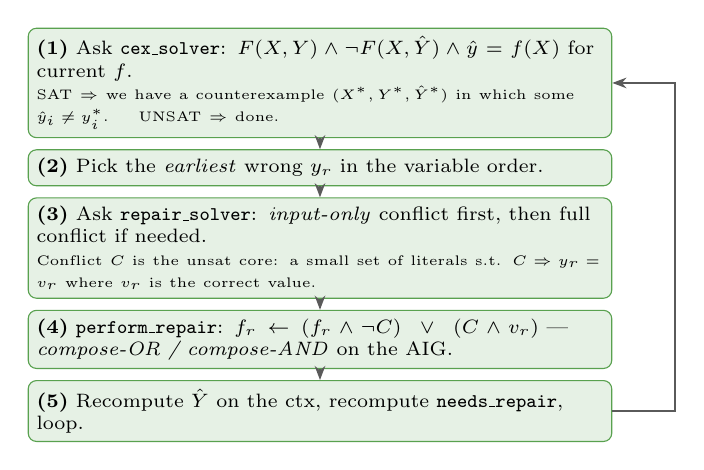
\begin{tikzpicture}[node distance=1.4mm]
\node[sB, text width=72mm] (a) {\textbf{(1)} Ask \texttt{cex\_solver}:
   $F(X,Y) \wedge \neg F(X,\hat Y) \wedge \hat y = f(X)$ for current $f$.\\
   {\tiny SAT $\Rightarrow$ we have a counterexample $(X^*, Y^*, \hat Y^*)$ in which
   some $\hat y_i \neq y_i^*$. \quad UNSAT $\Rightarrow$ done.}};
\node[sB, below=of a, text width=72mm] (b) {\textbf{(2)} Pick the
   \emph{earliest} wrong $y_r$ in the variable order.};
\node[sB, below=of b, text width=72mm] (c) {\textbf{(3)} Ask \texttt{repair\_solver}:
   \emph{input-only} conflict first, then full conflict if needed.\\
   {\tiny Conflict $C$ is the unsat core: a small set of literals s.t.
   $C \Rightarrow y_r = v_r$ where $v_r$ is the correct value.}};
\node[sB, below=of c, text width=72mm] (d) {\textbf{(4)} \texttt{perform\_repair}:
   $f_r \leftarrow (f_r \wedge \neg C)\;\vee\;(C \wedge v_r)$
   --- \emph{compose-OR / compose-AND} on the AIG.};
\node[sB, below=of d, text width=72mm] (e) {\textbf{(5)} Recompute $\hat Y$ on the
   ctx, recompute \texttt{needs\_repair}, loop.};
\foreach \a/\b in {a/b, b/c, c/d, d/e}
  \draw[fl] (\a) -- (\b);
\draw[fl] (e.east) -- ++(8mm,0) |- (a.east);
\end{tikzpicture}
\end{center}
\vspace{-2mm}
\scriptsize Each loop turn fires \texttt{stats\_every=40} / \texttt{detailed\_stats\_every=200}
log lines. Variable order is fixed up front by \texttt{bve\_order} (minimises
back-edges) so that ``earliest wrong'' is well-defined and avoids the
cyclic-repair pitfall.
\end{frame}

% =========================================================================
\begin{frame}{Cool idea: Craig interpolants as a smarter conflict}
  The conflict $C$ from step (3) is one \alert{corner} of the input space
  where the current $f_r$ is wrong. The straightforward repair only
  excludes that corner.
  \medskip

  \textbf{Better:} compute a \alert{Craig interpolant}
  $I(X)$~\cite{craig1957, mcmillan2003interpolation}, \emph{over inputs
  only}, separating the UNSAT proof's $A$ side (this corner) from the $B$
  side (the formula). $I(X)$ generalises the conflict to the
  \emph{entire} must-flip region of input space, so one
  \texttt{compose\_or} captures many repairs at once.
  \medskip

  \textbf{Implementation} (\texttt{interp\_repair.cpp}):
  \begin{itemize}\setlength{\itemsep}{1pt}
    \item A fresh CaDiCaL instance per repair, with an
          \texttt{InterpTracerMcMillan} attached as a proof tracer.
    \item Walk the proof core (clauses reachable from the empty clause)
          and build the McMillan interpolant by hash-consed AIG
          composition.
    \item \alert{Always verify}: an $A \rightarrow I$ miter check. On any
          tracer reconstruction bug we fall back to the plain conflict
          clause --- never produce a wrong interpolant.
  \end{itemize}
  \medskip
  \scriptsize Same Craig-interpolant idea drives Stages 2--3 above; only
  the partition $(A,B)$ differs.
\end{frame}

% =========================================================================
\begin{frame}{AIG rewriting and AIG-to-CNF -- why they matter}
  \textbf{Manthan's hot loop is the SAT solver.} Every repair grows the
  candidate AIG for some $y_i$; every grown AIG must be Tseitin-encoded
  into \texttt{cex\_solver}. If we encoded naively, \texttt{cex\_solver}
  would balloon and dominate runtime.
  \medskip

  \textbf{\texttt{AIGRewriter} (\texttt{aig\_rewrite.cpp}).}
  Each repair round runs \texttt{simplify\_aig} + an optional rewrite
  pass: constant propagation, complement elimination, idempotence,
  absorption, AND/OR distribution, XOR simplification, structural
  hash-consing, and \alert{FRAIG-lite SAT-sweeping}~\cite{mishchenko2005fraiging}.
  \medskip

  \begin{exampleblock}{\small Log: rewrite shrinks the AIG before encoding}
  \scriptsize
  \texttt{[aig-rewrite] nodes: 13290 $\rightarrow$ 11354
   (14.6\% reduction) absorption: 263 distrib: 842 hash\_hits: 190144}
  \end{exampleblock}
  \medskip

  \textbf{\texttt{AIGToCNF} (\texttt{aig\_to\_cnf.h}).}  K-ary AND/OR
  fusion, De Morgan flattening (free in the input-edge-neg model),
  ITE / MUX3 detection, and \emph{cut-CNF}~\cite{een2007applying} encoding for
  small cones.  One encoder per formula (cross-formula caching is
  unsound) --- caught by a per-formula AIG-vs-clauses miter under
  \texttt{SLOW\_DEBUG}.
\end{frame}

% =========================================================================
\begin{frame}{A worked example -- \texttt{bobtuint07neg}}
  \begin{center}\small
  \begin{tabular}{@{}lrrr@{}}
    \toprule
    Stage              & defined this stage & still to-define & wall time \\
    \midrule
    initial (after Puura) & ---                 & 1204             & --- \\
    \;\;synth-BVE         & ---                 & 353              & --- \\
    autarky               & 0                   & 353              & 0.01\,s \\
    extend                & 108                 & 245              & 0.04\,s \\
    backward-round-synth  & 99                  & 146              & 0.07\,s \\
    unate\_def            & 1                   & 145              & 1.02\,s \\
    \midrule
    Manthan (\texttt{bve} strategy) & \textbf{145}        & \textbf{0}       & 4.62\,s \\
    \bottomrule
  \end{tabular}
  \end{center}
  \medskip

  \begin{itemize}
    \item \textbf{Cheap stages first.} 209 of 353 vars defined before
          Manthan starts --- Manthan only handles the hard 145.
    \item \textbf{Manthan stats.} 1864 repairs in 1631 loops; 24\%
          repair-solver cache-hit rate; conflict size avg 8.96 lits.
    \item \textbf{Time breakdown.} 39\% in \texttt{cex\_finding},
          21\% in \texttt{find\_conflict}, 22\% in \texttt{recompute\_y\_hat}
          --- SAT calls and AIG bookkeeping dominate.
  \end{itemize}
\end{frame}

% =========================================================================
\begin{frame}{Takeaways}
  \begin{itemize}\setlength{\itemsep}{2pt}
    \item Arjun \emph{synthesises} Boolean functions on a Puura-simplified
          CNF: input / to-define / backward-defined is the only data
          model you need to follow the code.
    \item \textbf{Defining stages in cost order:} BVE-for-synth $\to$
          autarky $\to$ extend $\to$ backward $\to$ unate (def + conditional)
          $\to$ Manthan. Each stage runs only on what its predecessors left.
    \item \textbf{The duplication trick} (doubled CNF, ask whether the two
          copies can disagree) plus \textbf{Craig
          interpolation}~\cite{craig1957} via a CaDiCaL proof tracer
          turns each UNSAT witness into a working AIG.
    \item \textbf{Manthan} (CEGAR) handles the residue: BVE-style initial
          guess, CMSGen samples, CryptoMiniSat-backed repair solver,
          conflict (or interpolant) generalisation, AIG \texttt{compose}
          repair.
    \item \textbf{AIGRewriter + AIGToCNF} are the unsung heroes:
          they keep the cex-solver small so the CEGAR loop stays fast.
  \end{itemize}
\end{frame}

% =========================================================================
\begin{frame}[allowframebreaks]{References}
  \scriptsize
  \begin{thebibliography}{99}
    \setbeamertemplate{bibliography item}{}

    \bibitem{golia2020manthan} Priyanka Golia, Subhajit Roy, Kuldeep S.\ Meel.
      \emph{Manthan: A Data-Driven Approach for Boolean Function Synthesis.}
      CAV 2020.

    \bibitem{golia2021engineering} Priyanka Golia, Friedrich Slivovsky,
      Subhajit Roy, Kuldeep S.\ Meel.
      \emph{Engineering an Efficient Boolean Functional Synthesis Engine.}
      ICCAD 2021.

    \bibitem{liffiton2008} Mark H.\ Liffiton, Karem A.\ Sakallah.
      \emph{Searching for Autarkies to Trim Unsatisfiable Clause Sets.}
      SAT 2008.

    \bibitem{craig1957} William Craig.
      \emph{Three uses of the Herbrand–Gentzen theorem in relating model
      theory and proof theory.}  J.\ Symbolic Logic, 1957.

    \bibitem{mcmillan2003interpolation} Kenneth L.\ McMillan.
      \emph{Interpolation and SAT-based model checking.}  CAV 2003.

    \bibitem{jiang2009interpolating} Jie-Hong Roland Jiang, Hsuan-Po Lin,
      Wei-Lun Hung.
      \emph{Interpolating Functions from Large Boolean Relations.}
      ICCAD 2009.

    \bibitem{biere2019cadical} Armin Biere.
      \emph{CaDiCaL at the SAT Race 2019.}
      SAT Race 2019.

    \bibitem{soos2009cryptominisat} Mate Soos, Karsten Nohl,
      Claude Castelluccia.
      \emph{Extending SAT Solvers to Cryptographic Problems
      (CryptoMiniSat).}  SAT 2009.

    \bibitem{golia2021cmsgen} Priyanka Golia, Mate Soos, Sourav Chakraborty,
      Kuldeep S.\ Meel.
      \emph{Designing Samplers is Easy: The Boon of Testers (CMSGen).}
      FMCAD 2021.

    \bibitem{mishchenko2005fraiging} Alan Mishchenko, Satrajit Chatterjee,
      Roland Jiang, Robert K.\ Brayton.
      \emph{FRAIGs: A Unifying Representation for Logic Synthesis and
      Verification.}  ERL Technical Report, UC Berkeley, 2005.

    \bibitem{een2007applying} Niklas Eén, Alan Mishchenko, Niklas Sörensson.
      \emph{Applying Logic Synthesis for Speeding Up SAT.}  SAT 2007.

    \bibitem{korhonen2021integrating} Tuukka Korhonen, Matti Järvisalo.
      \emph{Integrating Tree Decompositions into Decision Heuristics of
      Propositional Model Counters (SharpSAT-td).}  CP 2021.

    \bibitem{niemetz2012b} Aina Niemetz, Mathias Preiner, Florian Lonsing,
      Martina Seidl, Armin Biere.
      \emph{Resolution-Based Certificate Extraction for QBF (DepQBF).}
      SAT 2012.

    \bibitem{john2015efficient} Ajith K.\ John, Shetal Shah, Supratik
      Chakraborty, Ashutosh Trivedi, S.\ Akshay.
      \emph{Skolem Functions for Factored Formulas.}  FMCAD 2015.

    \bibitem{durand2025fbcounting} Arijit Shaw, Kuldeep S.\ Meel.
      \emph{Counting on Definability: Tools and Tactics for Projected
      Model Counting.}  Recent work building on the Arjun
      definability ideas.

    \bibitem{soos2019bird} Mate Soos, Kuldeep S.\ Meel.
      \emph{BIRD: Engineering an Efficient CNF-XOR SAT Solver and Its
      Applications to Approximate Model Counting.}  AAAI 2019.

    \bibitem{soos2020bird} Mate Soos, Stephan Gocht, Kuldeep S.\ Meel.
      \emph{Tinted, Detached, and Lazy CNF-XOR Solving and Its
      Applications to Counting and Sampling.}  CAV 2020.
  \end{thebibliography}
\end{frame}

\end{document}
